\section{Tolerange} \label{sec:tolerange}

\Tolerange~toma como entrada también un modelo nominal y su implementación tolerante a fallas, esta vez siendo sistemas estocásticos, 
y produce como salida el número esperado de hitos acumulados que la implementación es capaz de preservar bajo un conjunto de fallas consideradas, esto es un valor en el intervalo $[0,\infty)$. Para asegurar que este valor está bien definido debemos asumir que la probabilidad de que el sistema eventualmente entre a un estado de falla es $1$. También asumimos que el ambiente juega de manera strong fair (si una acción o falla está habilitada con infinita frecuencia, entonces va a ocurrir con infinita frecuencia). A este tipo de sistemas los denominamos \emph{almost-surely failing bajo fairness} en el capítulo anterior. La herramienta puede verificar automáticamente si el juego derivado de los modelos es de este tipo.

Al igual que en {\MaskD}, un programa es una colección de procesos, donde cada uno está compuesto por una colección de acciones etiquetadas, esta vez de la forma: \verb"[Label]<reward>Guard->[P]Command++[Q]Command", donde: \verb"Guard" es una condición lógica sobre el estado actual del programa; \verb"Command" es 
una colección de asignaciones; \verb"Label" es el nombre de la acción; el entero positivo  \verb"reward" es 
opcional, y establece que la ejecución de esta acción cuenta como un ``hito'' de valor \verb"reward"; y \verb"++" es el operador de elección probabilista (aquí \verb"P" y \verb"Q" son las probabilidades correspondientes a cada rama de la elección; pueden haber varias ramas, siempre y cuando la suma de sus probabilidades sea $1$).
Al igual que antes, el lenguaje permite etiquetar a las acciones como \verb"faulty" para indicar que representan fallas. La gramática completa para el lenguaje de modelado se encuentra en el Apéndice~\ref{cap:appendix2}.

\iffalse
Para poder computar el número esperado de hitos logrados por la implementación, la herramienta utiliza nociones que vienen de la teoría de juegos.
More precisely,  first, we define a stochastic masking simulation game for any given nominal and fault-tolerant implementation model.
The basis of the game is similar to a probabilistic bisimulation game \cite{Stirling98}, and it is played by two players, 
named for convenience the Refuter ($\Refuter$) and the Verifier ($\Verifier$). The Verifier 
wants to prove that $s$ (a state of the specification) and $t$ (a state of the implementation) are \emph{probabilistic masking similar}, 
and the Refuter intends to disprove that.
The game starts from the pair of states $(s, t)$ and the following steps are repeated:
\begin{enumerate}
\item[1)] $\Refuter$ chooses either an action in the nominal model or an action in the implementation,  these actions have associated a probabilistic distribution,  which selects a next game state with certain probability.
Note that $\Refuter$ may select a fault.   Let $(a,\mu)$ be the action and distribution selected by $\Refuter$,
%  $\Refuter$ chooses either a transition $s \xrightarrow{a} \mu$ from
%  the nominal model or a transition $s' \xrightarrow{a} \mu'$ from the
%  implementation;
\item[2a)] If $a$ is not a fault,  $\Verifier$ has to match this with an action and a corresponding probabilistic distribution in the opposite model (say $(a,\mu')$),
it also selects a weighting function \cite{JonssonLarsen91} for $(\mu, \mu')$ (a function stating how the probabilities of both distributions are related).
\item[2b)]
  If $a$ is a fault,  $\Verifier$ can only select the Dirac
  distribution,  which gives probability $1$ to select as next state the actual state,   she also chooses the unique weighting function for
  $(\mu, \Dirac_{s})$. Intuitively, if  a fault occurs,  $\Verifier$ is obliged to mask the fault and cannot freely move in the nominal model.
\item[3)]
  The successor pair of states $(s',  t')$ is chosen  using the probabilities of the weighting function selected by $\Verifier$.
%% \item[1)] $\Refuter$ chooses action $a$ and distribution $\mu$ (resp. $\mu'$) such that $s \xrightarrow{a} \mu$ 
%% 		(resp. $s' \xrightarrow{a} \mu'$);
%% \item[2a)] If $a \notin \faults$, $\Verifier$ chooses a matching action $a$ and distribution $\mu'$ (resp. $\mu$) and 
%% 		a coupling $w$ such that $s' \xrightarrow{a} \mu'$ (resp. $s \xrightarrow{a} \mu$) and $w$ is coupling for $(\mu, \mu')$;
%% \item[2b)] If $a \in \faults$, $\Verifier$ selects the Dirac distribution  $\Dirac_{s}$ and a coupling $w$, such that 
%% 		$w$ is coupling for  $(\Dirac_{s}, \mu')$;
%% \item[3)] The successor pair of states $(t, t')$ is chosen probabilistically according to $w$.
\end{enumerate}
%
If the play continues forever, then the Verifier wins; otherwise, the
Refuter wins. %(Notice, in particular, that the Verifier loses if she cannot match a transition label, since choosing an arbitrary coupling is always possible.) Step 2b is the only one that differs from the usual
%bisimulation game.  This is needed because of the asymmetry produced by the
%transitions labeled with  faults. 
%Intuitively,  if the Refuter
%chooses to play a fault in the implementation, then the Verifier ought to
%mask the fault,  and she cannot freely move in the
%nominal model.  Summing up, the probabilistic step of a fault can only be
%matched by a Dirac distribution on the corresponding state of the specification. 

As explained above, we focus on those games
in which the refuter has probability $1$ of winning. Intuitively, this means that the system eventually will enter in an error state.  Furthermore, transitions could have associated a reward,  thus we obtain a quantitative version of these games: the Refuter intends to minimize the number of rewards collected by the Verifier, whereas the latter tries to maximize this number. Rewards are used to indicate the milestones that one  is interested in measuring. For instance, the number of ticks (discrete time) until the system fails.
\fi
%Accordingly, a bigger distance remarkably decreases fault-tolerance.
%We impleintroduce a game characterization of 
%masking simulation and we enrich the resulting games 
%with quantitative objectives to define the notion of 
%\emph{masking fault-tolerance distance}, 
%we start characterizing masking fault-tolerance via simulation relations between 
%two systems as defined in \cite{DemasiCMA17}. The first one acting as a specification 
%of the intended behavior (es decir, nominal model) and the 
%second one as the fault-tolerant implementation (es decir, the extended model with 
%faulty behavior).
%The existence of a masking relation implies that the implementation masks the faults.
%Afterwards, we introduce a game characterization of 
%masking simulation and we enrich the resulting games 
%with quantitative objectives to define the notion of 
%\emph{masking fault-tolerance distance}, 
%where the possible values of the game belong to the interval $[0,1]$. 
%In this game, the goal of the implementation is to mimic the behavior of the nominal model as much as possible.  In contrast, the
%nominal model tries to reach an error state as soon as possible. 
%Rewards are added to certain transitions in the game to reflect the fact that a fault was masked. 
%Thus, given a play (a maximal path in the game graph) a function $f_{\text{mask}}$ computes the value of the play: if it reaches the error state, the value is inversely proportional to the number of faults masked by the implementation; if the play is infinite,  it receives a value of $1$ indicating that the implementation was able to mask all the faults in the path. 
%The fault-tolerant implementation is masking fault-tolerant if the value of the game is $0$. Furthermore, the bigger the number, 
%the farther the masking distance between the fault-tolerant implementation and the specification. Accordingly, a bigger distance remarkably decreases fault-tolerance.
%Summing up,  as the final value gets closer to $1$ the implementation provides more masking fault-tolerance. 
%This value allows one to define a directed semi-metric, es decir, a function valuated in the interval $[0,1]$ that is transitive and it holds the triangle inequality, see \cite{CastroDDP18b} for the technical details.  
%The final value is given by the best play for the implementation given that the system uses an optimal play too.

\begin{figure}[t]
\centering
\begin{minipage}[t]{.47\textwidth}
\fontsize{10}{10}\selectfont\ttfamily
\begin{tabbing}
x\=xxxxxxxx\=xxxxxxxx\=xx\=xxx\= \kill    
Process NOMINAL \{\\[1ex]
\>v : INT; \\
\>s : INT;  		 \>\>// 0 = normal,\\ 
\>                   \>\>// 1 = refresh\\[1ex]
\>Initial: v==0 \&\& s==0;\\[1ex]
\>[write0]  !(s==1) -> v=0,s=0; \\
\>[write1]  !(s==1) -> v=1,s=0; \\[1ex]
\>[read0] !(s==1) \&\& v==0 -> v=v; \\
\>[read1] !(s==1) \&\& v==1 -> v=v; \\[1ex]
\>[tick] <1> s==0 -> 0.05 : s=1 \\
\>             \>\>++ 0.95 : v=v; \\[1ex]
\>[refresh] s==1 \&\& v==0 -> s=0, v=0; \\
\>[refresh] s==1 \&\& v==1 -> s=0, v=1; \\[1ex]
\}\\
\end{tabbing}
\end{minipage}
\caption{Modelo nominal para el ejemplo de la celda de memoria con refrescado.} \label{fig:exam_1_mem_cell_nom}
\vspace{-0.5cm}
\end{figure}

\begin{figure}[t]
\centering
\begin{minipage}[t]{.47\textwidth}
\fontsize{10}{10}\selectfont\ttfamily
\begin{tabbing}
x\=xxxxxxxx\=xxxxxxxx\=xx\=xxx\= \kill    
Process FAULTY \{\\[1ex]
\>v : INT; \\
\>s : INT;  		 \>\>// 0 = normal, 1 = refresh\\ 
\>                   \>\>// 2 = faulty\\[1ex]
\>Initial: v==0 \&\& s==0;\\[1ex]
\>[write0]  !(s==1) -> v=0,s=0; \\
\>[write1]  !(s==1) -> v=3,s=0; \\[1ex]
\>[read0] !(s==1) \&\& v<=1 -> v=v; \\
\>[read1] !(s==1) \&\& v>1 -> v=v; \\[1ex]
\>[tick] <1> s==0 -> 0.05 : s=1 \\
\>             \>\>++ 0.1 : s=2 \\
\>             \>\>++ 0.85 : v=v; \\
\>[tick] <1> s==2 -> 0.05 : s=1 \\
\>             \>\>++ 0.95 : v=v; \\[1ex]
\>[refresh] s==1 \&\& v<=0 -> s=0, v=0; \\
\>[refresh] s==1 \&\& v>1 -> s=0, v=3; \\[1ex]
\>[f] faulty s==2 \&\& v<3 -> s=0, v=v+1; \\
\>[f] faulty s==2 \&\& v>=3 -> s=0, v=2; \\
\>[f] faulty s==2 \&\& v>0 -> s=0, v=v-1; \\
\>[f] faulty s==2 \&\& v<=0 -> s=0, v=1; \\[1ex]
\}\\
\end{tabbing}
\end{minipage}
\vspace{-0.5cm}
\caption{Modelo de una implementación tolerante a fallas para el ejemplo de la celda de memoria con refrescado.} \label{fig:exam_1_mem_cell_ft}
\vspace{-0.5cm}
\end{figure}

Consideremos el ejemplo de la celda de memoria del Capítulo~\ref{cap:maskProb}. 
Las Figuras~\ref{fig:exam_1_mem_cell_nom} y  \ref{fig:exam_1_mem_cell_ft} muestran los procesos que representan al modelo nominal y la implementación tolerante a fallas, respectivamente. 
Las acciones $\texttt{read}i$
y $\texttt{write}i$ (para $i=0,1$) representan las acciones de lectura y escritura para el valor $i$.  El bit almacenado en la memoria está guardado en la variable~\texttt{v}.  La acción \texttt{tick} marca el paso de una unidad de tiempo y, con probabilidad \texttt{0.05}, habilita una acción de refrescado \texttt{refresh}). La variable \texttt{s}
indica si el sistema está en modo lectura/escritura, o produciendo un refrescado.
Una falla potencial en este escenario ocurre cuando una celda cambia de valor inesperadamente (e.g., como consecuencia de una interferencia electromagnética).
En la práctica, la ocurrencia de tal error tiene una cierta probabilidad. Nuevamente usamos  \emph{redundancia} para lidiar con estas fallas, %for instance
e.g., utilizando tres bits en lugar de uno. Luego, las operaciones de escritura se ejecutan simultáneamente sobre los tres bits mientras que una lectura retorna el valor de la mayoría.
El modelo de la Figura~\ref{fig:exam_1_mem_cell_ft} modela una implementación con triple redundancia y con las fallas mencionadas.  Ahora la variable \texttt{v} cuenta la cantidad de votos para el valor 1. Además de habilitar la acción de refrescado, un \texttt{tick} también puede habilitar la ocurrencia de una falla con probabilidad \texttt{0.1}.
%
La variable \texttt{s} ahora agrega un estado donde  puede ocurrir una falla ($\texttt{s}=2$).

\subsection{Arquitectura}
{\Tolerange} es un software de código abierto escrito en \textsf{Java}. 
%Documentation and installation instructions can be found at \cite{MaskD}. 
La arquitectura de la herramienta se muestra en la Figura~\ref{fig:arch_tolerange}.
\begin{figure}[ht]
    \centering
    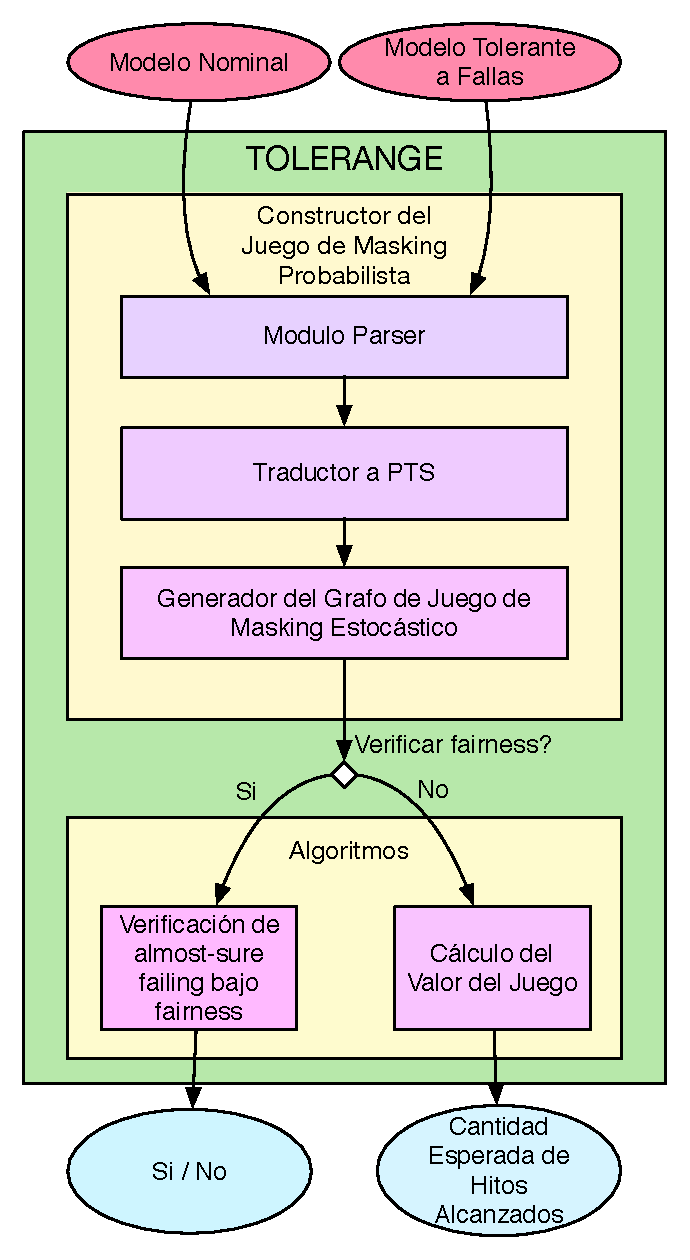
\includegraphics[scale=0.5]{Figs/TOLERANGE_ARCH.pdf}
    %\vspace{-0.4cm}
    \caption{Arquitectura de  \textsf{\Tolerange}.}\label{fig:arch_tolerange}
    %\vspace{-0.5cm}
\end{figure}
    En lo siguiente, describimos brevemente los componentes de la herramienta:
\begin{description}
    \item[Módulo Parser.] Realiza análisis sintáctico sobre los modelos de entrada, y produce estructuras de datos describiendo las entradas. Utiliza las librerías \textsf{Cup} y \textsf{JFlex}.
    \item[Traducción a PTS.] Los modelos obtenidos del parser se traducidos a Sistemas de Transición Probabilistas. 
    \item[Generación del Juego de Enmascaramiento Estocástico.] Se genera un juego de enmascaramiento estocástico para los PTS dados, donde las funciones de peso están capturadas simbólicamente a través de sistemas de ecuaciones (programación lineal).
    \item[Verificación de Terminación Bajo Fairness.] Se provee un algoritmo para verificar si un juego es casi-seguro terminante bajo fairness, consiste en computar los conjuntos predecesores en el grafo de juego simbólico. 
    \item[Cálculo del Valor del Juego (Algoritmo de Value Iteration).] El valor del juego puede ser computado solucionando una colección de ecuaciones funcionales a través de un algoritmo de \textit{value iteration}.
    Tomamos este valor como una medida de tolerancia a fallas.
    %This algorithm is polynomial in the game graph size.
\end{description}
\subsection{Modo de Uso}

El comando estándar para ejecutar {\Tolerange} en un sistema operativo Unix es:
\\ 
\\
 \verb"./Tolerange <options> <spec_path> <imp_path>"
\\
\\
    En este caso, la herramienta retorna la cantidad acumulada esperada de hitos logrados por la implementación.
Los comandos opcionales son: \verb"-f", para verificar si el juego es almost-sure failing bajo fairness;  \verb"-gurobi", el cual habilita {\Gurobi} \cite{gurobi} en lugar de {\SSC} \cite{SSC} para la programación lineal; y \verb"b=N" para establecer una cota superior de N para el valor del juego.
    Por defecto,  {\Tolerange} computa el valor del juego para las entradas dadas utilizando {\SSC} y una cota superior del número real máximo representable en {\Java}. 